% Paul Meyer-Rachner, paul@meyer-rachner.email 

%%%%%%%%%%%%%%%%%%%%%% DOCUMENT PARAMETERS %%%%%%%%%%%%%%%%%%%%%%%

\documentclass[usletter, 11pt]{extarticle}
\usepackage{style}
\usepackage{parskip}
\usepackage{fancyvrb}
\usepackage{soul}
\usepackage{mdframed}

\title{seizureDetection Matlab Tool User Guide}
\email{paul@meyer-rachner.email}

\newcommand{\seprule}[0]{\vspace{9pt} \hrule}


%%%%%%%%%%%%%%%%%%%%%% BEGIN DOCUMENT %%%%%%%%%%%%%%%%%%%%%%%%%%%%

\begin{document}

%%%%%%%%%%%%%%%%%%%%%% CUSTOMIZATION %%%%%%%%%%%%%%%%%%%%%%%%%%%%%

% space between bottom of text and footer
\setlength{\footskip}{20pt}
\setlength{\columnseprule}{0.2pt} 
\linespread{1.15}

% Title
\maketitle

\vspace{0.5cm}

%%%%%%%%%%%%%%%%%%%%%% BEGIN TEXT %%%%%%%%%%%%%%%%%%%%%%%%%%%%%%%%

\begin{mdframed}
\begin{tabular}{ll}
	\emph{Author:} & Paul Meyer-Rachner, paul@meyer-rachner.email \\
	\emph{Date:} & May 2018
\end{tabular}
\end{mdframed}

\tableofcontents

\newpage
\section{Introduction}

These MATLAB classes and functions were developed for the Berkeley MEng Capstone Project \emph{On-Chip Biosignal Computation for Health Monitoring} at the University of California, Berkeley Department of Electrical Engineering and Computer Science during the 2017-2018 academic year. The advisor was professor Rikky Muller. \\

The goal of the project was to develop a implantable microchip that monitors the brain's electrical activity (electroencephalogram or EEG) to detect seizures. This tool was developed while coming up with a detection algorithm that could reliably detect seizures while minimizing hardware complexity. \\

\begin{mdframed}
\textbf{\underline{Note:} The final project report should also be available to download at the same location as this tool. Reading it, especially the software part (section 2.1) of it will help understand this tool. Furthermore, all functions should have ample comments and the \texttt{main.m} file contains example of how to uses the functions and classes provided by this tool.}

\textbf{\ul{This documentation is not exhaustive, it is supposed to give an overview of the tool. Many functions in the code are not documented here (but there are ample comments within the code).}}
\end{mdframed}

\section{Tool overview}

The main component of the tool are 4 MATLAB classes:
\begin{itemize}
	\item The \texttt{Measurement} class holds raw EEG data.
	\item The \texttt{FeatureCalculation} class is used to extract different features from the data. It offers several functions to calculate that feature, further process it and visualize it. Every feature has it's own class that is a children of the FeatureCalculation class.
	\item The \texttt{FeatureMatrix} class serves to hold multiple FeatureCalculation objects inside a matrix. 
	\item The \texttt{MatrixDetection} class is used to detect seizures. It uses the information of all the features stored inside a \verb|FeatureMatrix| object to calculate a weighted sum that will be used to detect seizures. \\
\end{itemize}

The usual workflow is as follows:
\begin{enumerate}
	\item Create a Measurement object with some EEG data. This can be achieved either by downloading the data from iEEG.org using the function \verb|IEEG_getData| or manually creating a Measurement object with the appropriate data.
	\item Filter the data using the \verb|preprocess| function of the Measurement class. Then calculate different features and store those in a \verb|FeatureMatrix| object. This can be done by adapting the script \verb|generateMatrix|.
	\item Create a \verb|MatrixDetection| object and use it to detect seizures.
\end{enumerate}

%--------------------------------------------------------------------
\newpage
\section{The Measurement class}


The \verb|Measurement| class holds the EEG data and the location of the seizures.

The function \verb|IEEG_getData| allows to download data from the iEEG.org\footnote{\url{https://www.ieeg.org}} website (see section \ref{sec:ieeg_getdata}). 

\subsection{Class Properties}

The table below show the properties of the \texttt{Measurement} class. Some of these properties have their SetAcces set to protected, meaning it is not possible to modify them directly from outside the class. This is done to protect the integrity of the object by preventing accidental modification of important properties.

\begin{center}
	\begin{tabular}{p{4cm}|p{12cm}}
	\textbf{Name:} & \textbf{Description:} \\ \hline
	\texttt{Data}& holds the EEG data \\
	\texttt{Ts}& sampling time in seconds \\
	\texttt{Fs}& sampling frequency in Hz (equivalent to 1/Ts)\\
	 \texttt{Length}& length of the Data property in samples\\
	 \texttt{NumSeizures}& number of seizures present in the measurment\\
	 \texttt{SeizureStart}& a double array containing the start of each seizure in terms of samples\\
	 \texttt{SeizureEnd}& a double array containing the end of each seizure in terms of samples\\
	 \texttt{SeizureDuration}& the duration of each seizure in seconds\\
	 \texttt{Duration}& duration of the measurement in seconds\\
	 \texttt{isNaN}& a logical array that has the same length as the Data property. For some measurement, the original data contains NaN values. This results in issues when filtering the data. Thus the object is created, these NaN values are replaced with their nearest non NaN value, but their position is remembered so that the original NaN value can be set again at a later point.\\
	 \texttt{FilterOrder}& the order of the bandpass filter used to preprocess the data\\
	 \texttt{FilterFc1}& the lower cutoff frequency of the bandpass filter, in Hz\\
	 \texttt{FilterFc2}& the higher cutoff frequency of the bandpass filter, in Hz\\
	 \texttt{StudyName}& a string containing the original name of the study the data is coming from. This is mainly used to identify the data.\\
	 \texttt{StudyChannelNumber}& a double holding the channel number the data is coming from. This is mainly used to identify the data.\\
	 \texttt{StudyChannelName}& a string holding the identifier of the channel. This is mainly used to identify the data.\\
\end{tabular}

\end{center}

\subsection{Class methods}

\subsubsection{Constructor}

An instance of the Measurement class is created by calling the class constructor:
\begin{Verbatim}
	measurement = Measurement(data, Fs, seizureStart, seizureEnd, 'Name', 'Value')
\end{Verbatim}

It has 4 required input arguments. \verb|data| is the raw EEG data and \verb|Fs| the sampling frequency. \verb|seizureStart| and \verb|seizureEnd| are two vectors containing the start and end location in samples of each seizure.

Possible Name-Value pairs for customization are:
\begin{center}
	\begin{tabular}{p{4cm}|p{4cm}}
	\textbf{Name:} & \textbf{Type:} \\ \hline
	\texttt{StudyName} & char\\
	\texttt{StudyChannelNumber} & scalar double \\
	\texttt{StudyChannelName} & char \\
\end{tabular}
\end{center}

The \texttt{FilterOrder}, \verb|FilterFc1| and \texttt{FilterFc2} are initialized with default values 6, 1 Hz and 70 Hz respectively and can be changed once the object is created.

\subsubsection{Preprocess function}

The \verb|preprocess()| function filters the data using a Butterworth bandpass filter with order and cutoff frequencies specified in the object properties.  This function has no input arguments.

The filter object is created using MATLAB's builtin \verb|fdesign.bandpass| and \verb|design| functions. The resulting feature object is a second-order section implementation, meaning that several second order Butterworth filters are cascaded. For example, if original order is 6, then 3 second order sessions will be cascaded. This implementation reduces the hardware requirement of the filter and prevents the filter from becoming unstable due to the numerical instability introduced by the bilinear transformation in the filter design process.

\subsubsection{Downsample function}

The \verb|downsample(n)| function downsample the measurement by an integer factor. For example, if the original sampling frequency is 512 Hz, then after calling \verb|downsample(2)|, the sampling frequency will be 256 Hz. 

The function takes one input, \verb|n|, which is the downsampling factor. It has to be an integer, and the resulting frequency also has to be an integer. For example, a 512 Hz measurement cannot be downsampled by 3.

Internally, the MATLAB function \verb|decimate| is called, which applied an anti-aliasing lowpass filter to the data before downsampling it to avoid aliasing.

All object properties like \verb|seizureStart| are adjusted to the new sampling frequency.

\subsubsection{Cut function}

The function \verb|cut(startIndex, endIndex)| trims the measurement to the indices given as input parameters. The function issues a warning if seizures are removed from the data and throws an error if the start or end index are within a seizure. All object properties like \verb|seizureStart| and \verb|duration| are adjusted to the start and end. 

\subsubsection{Other functions}

The function \verb|plot()| plots the current EEG data. Seizures are plotted in red. If the measurement is very large, it will take a while to run and the resulting plot will not be very responsive when interacted with. \\

The function \verb|isSeizure(queryIndices)| return a logical array of the same size as the input argument \verb|queryIndices|. For every index inside \verb|queryIndices|, the output is \verb|True| if that index corresponds to a seizure in the measurement and \verb|False| otherwise.

%--------------------------------------------------------------------
\newpage
\section{The FeatureCalculation class and it's children}

The \verb|FeatureCalculation| class is an abstract class used to calculate one feature from the EEG data. It has 4 children that can be instantiated:
\begin{itemize}
	\item The \verb|LineLength| class to calculate the line length feature
	\item The \verb|NonlinearEnergy| class to calculate the nonlinear energy feature
	\item The \verb|Power| class to calculate power in the whole spectrum
	\item The \verb|SpectralBandPower| class to calculate the power in one spectral band
\end{itemize}
See appendix \ref{sec:formulas} for the mathematical formulas of how those features are implemented.

\subsection{Class Properties}

The table below show the properties of the \texttt{FeatureCalculation} class. As for the \verb|Measurement| class, some of these properties have their SetAcces set to protected. The term 'feature sample' refers to the update frequency or step size of the sliding window used to calculate the feature. For example, it is 0.2 seconds by default, meaning one feature sample is equivalent to 0.2 seconds and one new feature value will be calculated every 0.2 seconds.

\begin{center}
	\begin{longtable}{p{5cm}|p{12cm}}
	\textbf{Name:} & \textbf{Description:} \\ \hline
	\texttt{FeatureName} & the name of the feature \\
	\texttt{Value} & the value of the feature \\
        
    \texttt{CharacteristicCurve} &  holds an \verb|OperatingCharacteristicCurve object| (see section \ref{sec:roc})  \\
        
    \texttt{StudyName} & study name of original measurement, copied from the linked measurement \\
    \texttt{StudyChannelNumber} & channel number of original measurement, copied from the linked measurement \\
    \texttt{StudyChannelName} & identifier of the channel, copied from the linked measurement \\
    \texttt{BaselineWindowLength} & the length of the window over which the baseline is calculated, in term of feature samples \\
    \texttt{BaselineShift} & the amount of time the window over which the baseline is calculated is delayed, in term of feature samples\\
    \texttt{BaselineRefreshrate} & how often the baseline value is updated, in term of feature samples \\
    
    \texttt{ThresholdBaselineFactor} & factor by which the baseline is multiplied to obtain the threshold \\
    
    \texttt{LinkedMeasurement} & a handle (reference/link) to the \verb|Measurement| object that is being analysed \\
    
    \texttt{PlotHandle} & a handle to the plot of the feature (if there is one) \\
    \texttt{AxesHandle} & a handle array containing the axes handles of the plot (if there is one) \\
    
    \texttt{CostSensitivity} & factor for calculating cost of not detecting seizures when finding the best threshold \\
    \texttt{CostFalseAlarmRate} & factor for calculating cost of false alarms when finding the best threshold \\
    \texttt{SeizureHoldTime} & duration of a seizure for evaluation purpose in feature samples (see section \ref{sec:feat_calc_eval}) \\
    \texttt{Baseline} & feature value baseline, average of feature value over a longer window, used to calculate the threshold \\
    
    \texttt{StepSize} & update frequency of the sliding window, in terms of measurement samples (for example, if the sampling frequency of the measurement is 500Hz and the update frequency is 0.2s, then \verb|StepSize| will be 100)\\
    \texttt{WindowLength} & the length of the window used to calculate the feature value, in terms of measurement samples (for example, if the sampling frequency of the measurement is 500Hz and the update frequency is 1s, then \verb|WindowLength| will be 500)\\
    \texttt{Length} & total number of calculated values \\
    
    \texttt{SeizureStart} & start index of the seizures, in terms of feature samples \\
    \texttt{SeizureEnd} & end index of the seizures, in terms of feature samples \\
    \texttt{NumSeizures} & total number of seizures \\
    \texttt{MeasurementFs} & sampling rate of linked measurement, useful is case the link in the \verb|LinkedMeasurement| property is deleted \\
    \texttt{Duration} & duration of linked measurement, useful is case the link in the \verb|LinkedMeasurement| property is deleted \\
    
    \texttt{Sensitivity} & percentage of detected seizures \\
    \texttt{Specificity} & percentage of time above threshold outside of seizure areas \\
    \texttt{FalseAlarms} & number of false alarms \\
    \texttt{ThresholdCrossings} & number of times the feature value exceeded the threshold \\
    \texttt{FalseAlarmRate} & number of false alarms per hour \\
    \texttt{MissedSeizures} & locations of seizure that were not detected, in terms of feature samples \\
    \texttt{BitSeizureDetected} & Logical array, index \verb|BitSeizureDetected[i]| is \verb|True| when the $i$th seizure is detected by this feature and \verb|False| otherwise \\
    \texttt{ThresholdCrossedLocation} & indices where the feature value crossed the threshold, in terms of feature samples \\
    \texttt{FalseAlarmLocation} & indices of false alarms, in terms of feature samples 
	\end{longtable}
\end{center}

Additionally, the \verb|SpectralBandPower| has two additional properties:
\begin{itemize}
	\item \verb|FrequencyBounds| contains the upper and lower frequency limit in Hz of the band. It is also used as cutoff frequencies when filtering the data during the feature value calculation. 
	\item \verb|FilterOrder| is the order of the Butterworth bandpass filter used to filter the data
\end{itemize}

\subsection{Class Methods}

\subsubsection{Constructors}

The \verb|FeatureCalculation| is an abstract class and can therefore not be instanciated. 

The objects of the classes \verb|LineLength|, \verb|NonlinearEnergy| and \verb|Power| can be created by calling
\begin{Verbatim}
	linelength = LineLength(measurement, 'Name', 'Value')
	nonlinearEnergy = NonlinearEnergy(measurement, 'Name', 'Value')
	power = Power(measurement, 'Name', 'Value')
\end{Verbatim}
where measurement is a \verb|Measurement| object.

\newpage
Possible Name-Value pairs are: 

\begin{center}
	\begin{longtable}{p{5.5cm}|p{1.5cm}|p{1.5cm}|p{7.5cm}}
	\textbf{Name:} & \textbf{Type:} & \textbf{Default:} & \textbf{Description} \\ \hline
	\texttt{StepSize\_seconds} & double & 0.2 & defines by how much the sliding window is moved in seconds (equivalent to how often the sliding window is updated). This can be thought of as the feature sampling frequency.\\
	\texttt{WindowLength\_seconds} & double & 1 & the length of the sliding window in seconds \\
	\texttt{BaselineAverageTime\_seconds} & double & 180 & over what period of time the baseline is calculated, is seconds \\
	\texttt{AverageWindowShift\_seconds} & double & 120 & by how much the window over which the baseline is calculated is delayed, in seconds \\
	\texttt{BaselineRefreshRate\_seconds} & double & 30 & how often the baseline is recalculated/refreshed, in seconds \\
	\texttt{SeizureHoldTime\_seconds} & double & 60 & duration of a seizure for evaluation purpose in feature samples (see section \ref{sec:feat_calc_eval}) \\
	\texttt{CostSensitivity} & double & 50 & factor for calculating cost of not detecting seizures when finding the best threshold \\
	\texttt{CostFalseAlarmRate} & double & 1 & factor for calculating cost of having many false alarms when finding the best threshold \\
	\texttt{ThresholdBaselineFactor} & double & 5 & factor by which the baseline is multiplied to obtain the threshold	
\end{longtable}
\end{center}

Instances of the \verb|SpectralBandPower| class are created by calling
\begin{Verbatim}
	thetaBand = SpectralBandPower(measurement, bandName, frequencyBounds)
\end{Verbatim}
where \verb|bandName| is a char containing the name of that band and \verb|frequencyBounds| an double array of length 2 containing the upper and lower limit of the band in Hz. Additionally, the order of the filter used to filter the data can be passed as a Name-Value pair, for example
\begin{Verbatim}
	thetaBand = SpectralBandPower(measurement, 'ThetaBand', [4 8], 'FilterOrder', 6)
\end{Verbatim}

The constructors of all 4 children class convert the parameters specified by the Name-Value pairs (or the default values) from duration in seconds to length in feature samples.

\subsubsection{Calculate function}

The \verb|calculate()| function calculates the feature value using the filtered data in the \verb|Measurement| object linked to it. It does not take any input arguments. It calls the \verb|calculateFeatureValue| that has to be implemented by the children classes. The \verb|calculateFeatureValue| used the MATLAB builtin function \verb|movmean| since it allows for a fast calculation of the feature value.

The \verb|calculate| function also calculates the baseline. The baseline is the average of the feature value over a longer window (180 seconds by default). This window is however delayed by a certain amount (120 seconds by default). For example, the baseline corresponding to time $t$ will be calculated by averaging the feature value from time $t - 300$ to time $t - 120$.

\subsubsection{Evaluate function} \label{sec:feat_calc_eval}

The \verb|evaluate()| function calculates the seizure detection metrics using the current value of the \linebreak \verb|ThresholdBaselineFactor| property. See appendix \ref{sec:metrics} for a definition of some of the metrics calculated. It does not take any input arguments.

One seizure counts as detected when the feature value crosses the threshold at least once during the seizure time.

One false alarm is defined as the feature value crossing the threshold outside of seizure areas. However, if the threshold is crossed repeatedly within a short timeframe (specified by the \verb|SeizureHoldTime|) property, only the first threshold crossing is marked as a false alarm and all others are ignored. This is to avoid generating too many false alarms when the feature values oscillates around the threshold. This also mirrors the behavior of the actual seizure detection chip, where a response is trigger when a seizure is detected. This response cannot be trigged in too short time intervals. Thus, internally, the function \verb|calculateFalseAlarmLocation| is called to identify and delete such redundant false alarms.

\subsubsection{CalculateOperatingCharacteristicCurve function}

The \verb|calculateOperatingCharacteristicCurve()| calculates the sensitivity and false alarm rate for different \verb|ThresholdBaselineFactor| and uses the result to create a \verb|OperatingCharacteristicCurve| object (see section \ref{sec:roc}) that is then stored in the \verb|CharacteristicCurve| property. It does not take any input arguments.

The sensitivities and false alarm rates are calculated by calling the \verb|evaluate| function repeatedly for different values of \verb|ThresholdBaselineFactor|.

\subsubsection{FindBestThreshold function} 

The \verb|findBestThreshold()| function finds the value of \verb|ThresholdBaselineFactor| that minimizes a cost function and stores it inside that property. It does not take any input arguments. The cost function is currently defined by 
$$\text{Cost} = \text{CostSensitivity}\times(1-\text{Sensitivity})^2 + \text{CostSensitivity}\times\text{FalseAlarmRate}.$$

The \verb|findBestThreshold| function uses the sensitivities and false alarm rates stored in the
\texttt{Operating\-Charac\-teristic\-Curve} object to calculate the cost, therefore the function \texttt{calculate\-Operating\-Charac\-teristic\-Curve} must be called before the \verb|findBestThreshold| function.

\subsubsection{Plot function} \label{sec:feature_plot}

The \verb|plot(flags)| function plots the feature value. Several flags can be passed as chars to the function to modify how the plot looks:
\begin{itemize}
	\item \verb|'Measurement'|: also plot the linked measurement data. This will results in a plot with two subplots and can be slow if the measurement is large.
	\item \verb|'Threshold'|: plots the threshold in addition the feature value
	\item \verb|'Baseline'|: plots the baseline in addition the feature value
	\item \verb|'Mark'|: mark missed seizures and false alarms on the plot
	\item \verb|'Bare'|: removes legends and ticks and other annotations from the plot
\end{itemize}

For example, the plot in figure \ref{fig:plot_feature} was created by calling the command
\begin{Verbatim}
	linelength.plot('Measurement', 'Threshold', 'Mark').
\end{Verbatim}

\begin{figure}[!h]
	\centering
	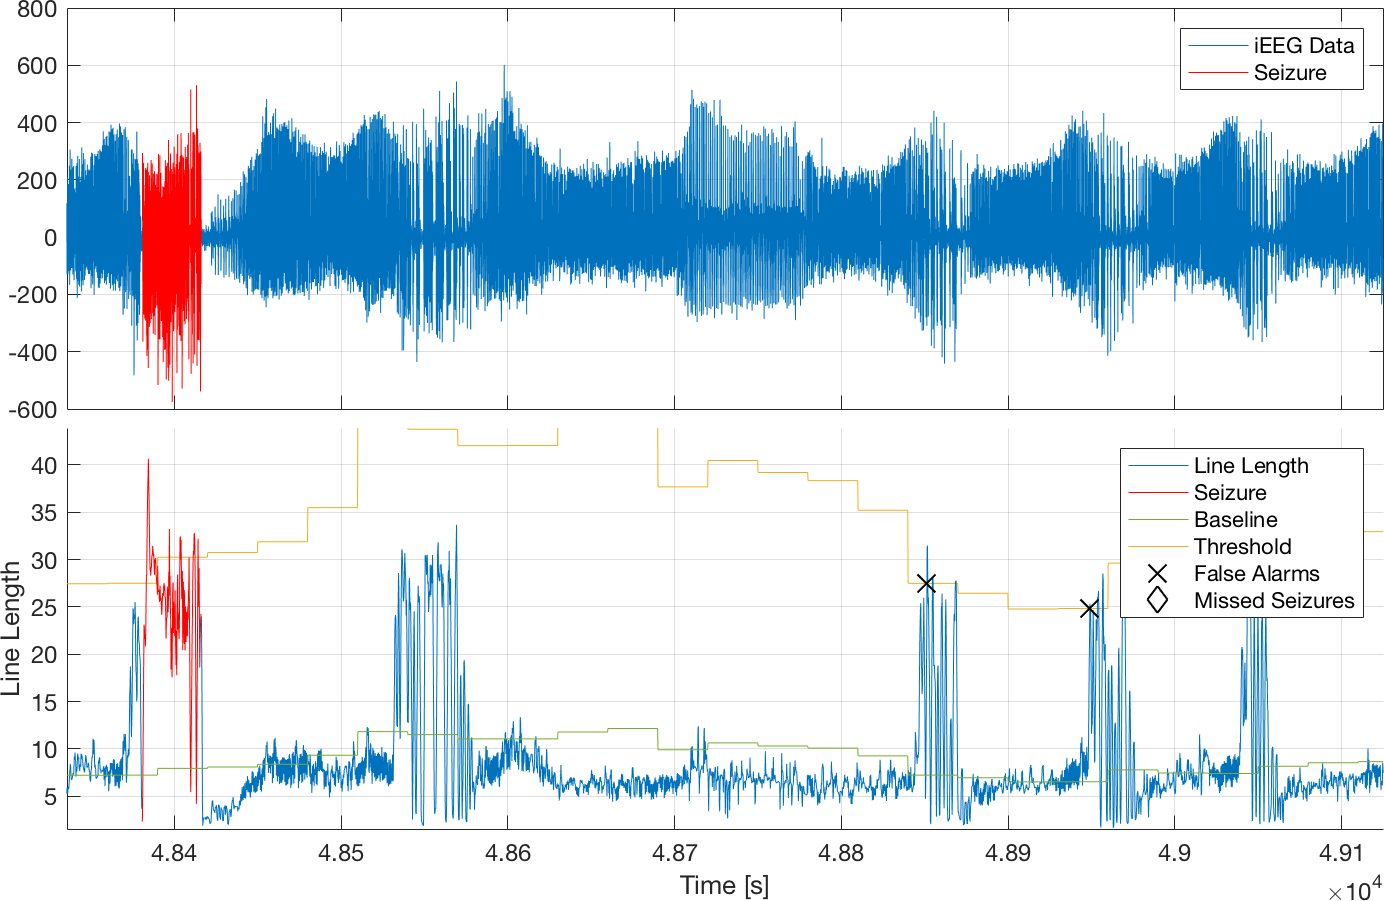
\includegraphics[width = \textwidth]{img/example_feature_plot}
	\caption{Example of a plot generated with the \texttt{plot} function of the \texttt{FeatureCalculation} class.}
	\label{fig:plot_feature}
\end{figure}

%--------------------------------------------------------------------
\clearpage
\section{The FeatureMatrix class}

The \verb|FeatureMatrix| class provides a container to store \verb|FeatureCalculation| objects (more precisely, it's children object) inside a matrix.

A feature matrix object can be generated by adapting the \verb|generateMatrix| script.

\subsection{Class Properties}

All the properties of the \verb|FeatureMatrix| class are private.

\begin{center}
	\begin{longtable}{p{5cm}|p{12cm}}
	\textbf{Name:} & \textbf{Description:} \\ \hline
	\texttt{FeatureNames} & a cell array of strings containing the names of the features \\
	\texttt{Matrix} & the actual feature matrix, it is a cell array of size number of channels $\times$ number of features \\
	\texttt{NumChannels} & number of channels (and therefore rows) in the feature matrix \\
	\texttt{NumFeatures} & number of different features (and therefore columns) in the feature matrix \\
	\texttt{NumElements} & the total number of elements in the matrix (equals to number of rows $\times$ number of columns) \\
	\texttt{FeatureLength} & the length in samples of one feature \\
	\texttt{NumSeizures} & the number of seizures in one feature \\
	\texttt{SensitivityMatrix} & a double matrix of the same size as \verb|Matrix| that holds the sensitivity of each feature \\
	\texttt{SpecificityMatrix} & a double matrix of the same size as \verb|Matrix| that holds the specificity of each feature \\
	\texttt{FalseAlarmRateMatrix} & a double matrix of the same size as \verb|Matrix| that holds the false alarm rate of each feature \\
	\texttt{AreaMatrix} & a double matrix of the same size as \verb|Matrix| that holds the area under curve between a false alarm rate of 0 and 1 of each feature \\
	\texttt{FlagMatrix} & a 3-dimensional matrix of logical values. Index $[i, j, k]$ is true when for channel $i$ feature $j$ is above it's threshold at index $k$. The dimension is [number of channel $\times$ number of features $\times$ length of one feature] \\
	\texttt{BitSeizureDetectedMatrix} & a 3-dimensional matrix of logical values. Index $[i, j, k]$ is true when for channel $i$ feature $j$ detected seizure number $k$. The dimension is [number of channel $\times$ number of features $\times$ number of seizures]
	\end{longtable} 
\end{center}

\subsection{Class Methods}

\subsubsection{Constructor}

The construct of the \verb|FeatureMatrix| class has two required input arguments, the number of channels \verb|numChannels| which is a double and a cell array of string containing the names of the features that will be included in the feature matrix.
\begin{Verbatim}
	matrix = FeatureMatrix(numChannels, featureNames)	
\end{Verbatim}

The feature names have to match exactly with the \verb|FeatureName| properties of the features classes. 

\subsubsection{Filling the feature matrix entries}

An single element can be added to the matrix by the following command:
\begin{Verbatim}
	matrix.setElement(indexChannel, feature)	
\end{Verbatim}
where \verb|indexChannel| is a double corresponding to the channel number and \verb|feature| is a feature calculation object. The \verb|setElement| function will compare the \verb|FeatureName| property of the object passed as input argument and compare it with the \verb|FeatureNames| property of the \verb|FeatureMatrix| object to determine the correct insertion column. This is why when instantiating a \verb|FeatureMatrix| object, the feature names passed to the constructor have to match the names of the feature objects.

\subsubsection{Filling the other matrices}

The matrices \verb|SensitivityMatrix|, \verb|SpecificityMatrix|, \verb|FlagMatrix| and \verb|BitSeizureDetectedMatrix| can be filled by calling the function \verb|fillMatrices()|. These matrices are mainly used for the matrix (weighted sum) seizure detection.

The matrix \verb|AreaMatrix| can be filled by calling the \verb|fillAreaMatrix()| function. This requires all elements inside the feature matrix to have their \verb|CharacteristicCurve| property calculated.

\subsubsection{Plotting all features in on channel or all features of one kind}

The function \verb|plot(strWhat, index)| plots either all features in one channel if the input argument \verb|strWhat| is set to \verb|'feature'| or one specific feature for all channels if it is set to \verb|'channel'|. The feature or channel to plot is determined by the second input argument \verb|index|. For example, to plot all features of channel 1 call \verb|plot('channel', 1)| and to plot the nonlinear energy feature for all channels call \verb|plot('feature', '2')| (assuming the nonlinear feature corresponds to the seconds column). As with the \verb|plot| function of the \texttt{FeatureCalcu\-lation} object, it is possible to pass additional flags to the function to customize the appearance of the plot (see section \ref{sec:feature_plot}). The possible flags are:
\begin{itemize}
	\item \verb|'Threshold'|: plots the threshold in addition the feature value
	\item \verb|'Baseline'|: plots the baseline in addition the feature value
	\item \verb|'Mark'|: mark missed seizures and false alarms on the plot
	\item \verb|'Bare'|: removes legends and ticks and other annotations from the plot
\end{itemize}

For example, the plot in figure \ref{fig:plot_matrix} was created using the command
\begin{Verbatim}
	matrix.plot('feature', 1, 'Threshold', 'Mark', 'Bare').
\end{Verbatim}


\begin{figure}[!h]
	\centering
	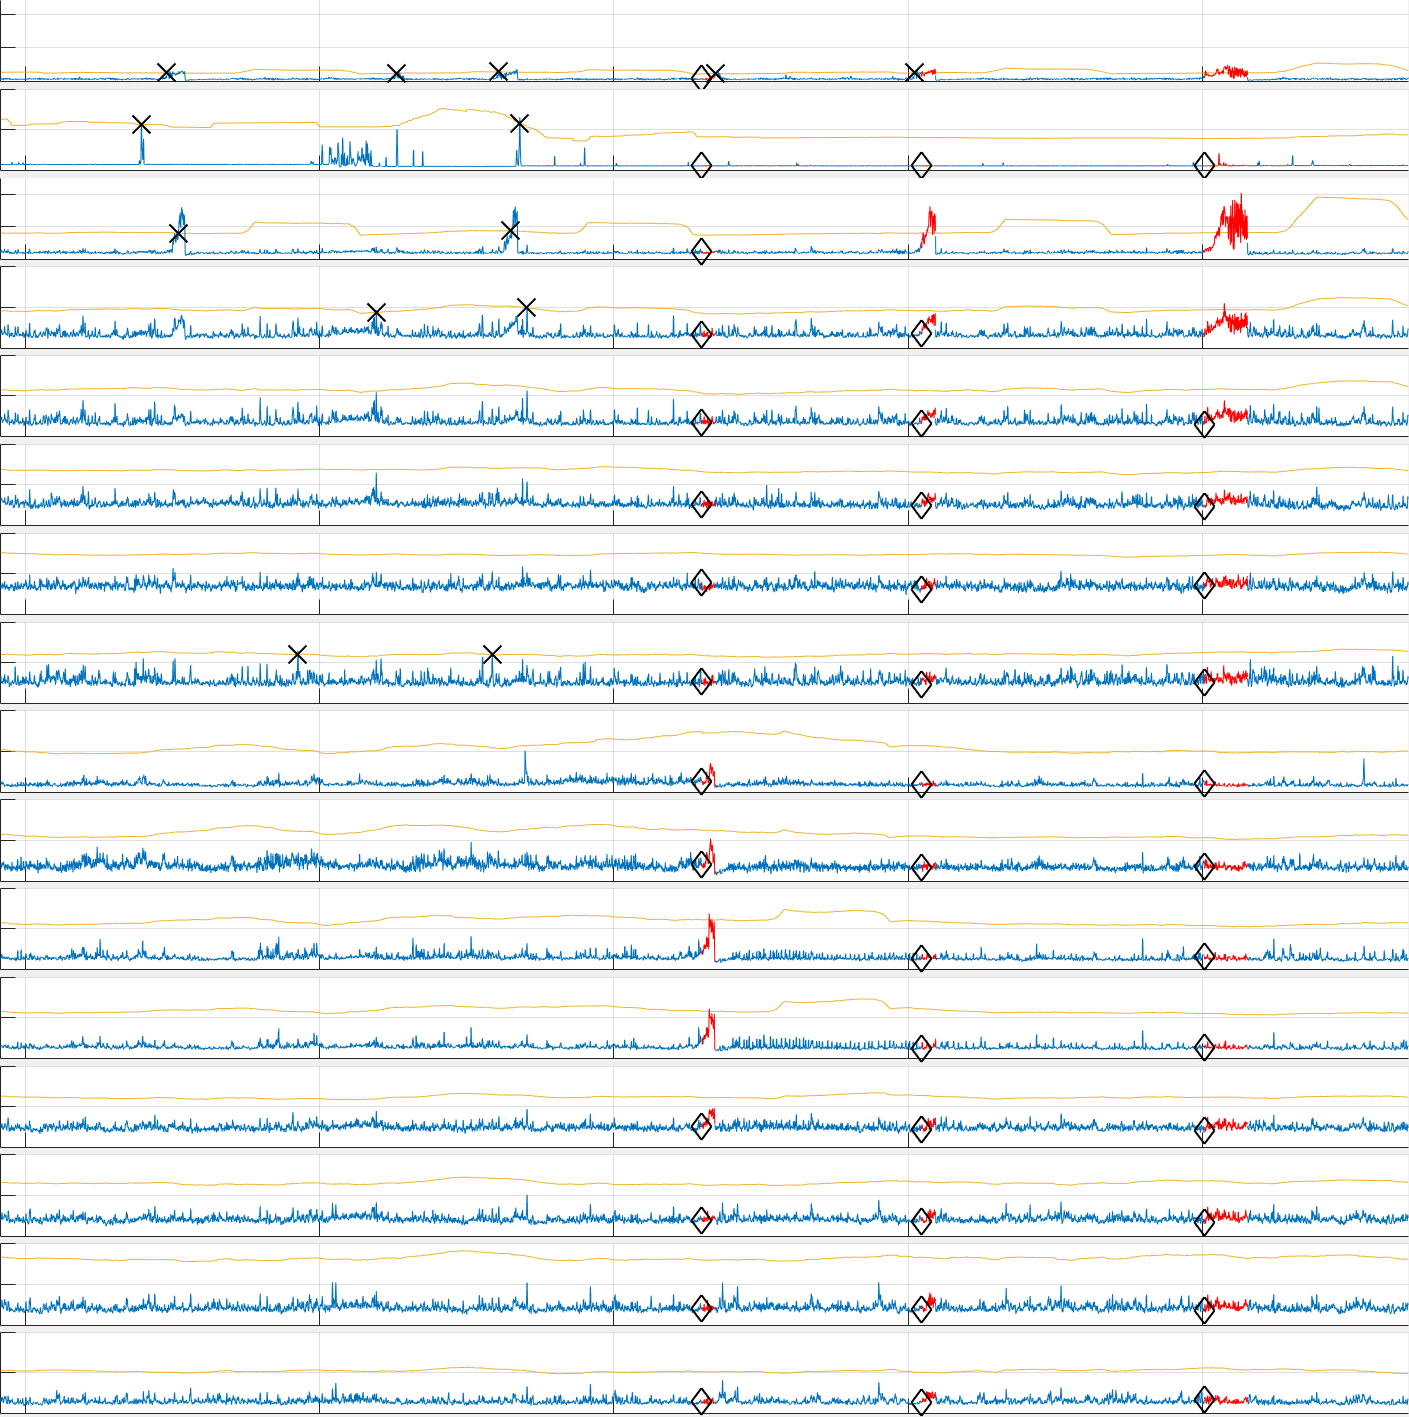
\includegraphics[width = \textwidth]{img/example_matrix_plot}
	\caption{Example of a plot generated with the \texttt{plot} function of the \texttt{FeatureMatrix} class. The plot is not annotated because the flag \texttt{'Bare'} was used.}
	\label{fig:plot_matrix}
\end{figure}

%--------------------------------------------------------------------
\clearpage
\section{The MatrixDetection class and it's children}

The \verb|MatrixDetection| class is a class designed to handle the weighted sum detection of seizures. The idea is to assign a weight to every feature of the feature matrix inside the \verb|FeatureMatrix| class. The weight is determined by how good that feature is at detecting seizures. For more information on how and why this is done, please read the Capstone Project Final Report that is also available with this user guide. 

The class can be instantiated on it's own, but usually one of it's children is used. Currently, there is only one children of this class, the \verb|MatrixDetection_LinearRegression| class.

This class is in many aspects similar to the \verb|FeatureCalculation| class.

\subsection{Class properties}

This class has many of the properties of the \verb|FeatureCalculation| class.

\begin{center}
	\begin{longtable}{p{5cm}|p{12cm}}
	\textbf{Name:} & \textbf{Description:} \\ \hline
	\texttt{WeightMatrix} & a double matrix that holds the weight of every element of the feature matrix \\
	\texttt{Name} & name of the object \\
	\texttt{Value} & the value of the weighted sum \\
    \texttt{CharacteristicCurve} &  holds an \verb|OperatingCharacteristicCurve object| (see section \ref{sec:roc})  \\
        
    
    \texttt{Threshold} & the threshold used for detection. Unlike in the \verb|FeatureCalculation| class, this is a fixed value as there is no baseline in the \verb|MatrixDetection| class. \\
    
    \texttt{LinkedMatrix} & a handle (reference/link) to the \verb|FeatureMatrix| object that is being analysed \\
    \texttt{NumElements} & number of elements in the linked feature matrix \\
    
    \texttt{CostSensitivity} & factor for calculating cost of not detecting seizures when finding the best threshold \\
    \texttt{CostFalseAlarmRate} & factor for calculating cost of false alarms when finding the best threshold \\
    \texttt{SeizureHoldTime} & duration of a seizure for evaluation purpose in feature samples (see section \ref{sec:feat_calc_eval}) \\

    \texttt{FeatureLength} & the length of the individual features, also the length of the weighted sum value \\
    
    \texttt{SeizureStart} & start index of the seizures, in terms of feature samples \\
    \texttt{SeizureEnd} & end index of the seizures, in terms of feature samples \\
    \texttt{NumSeizures} & total number of seizures \\
	
    
    \texttt{Sensitivity} & percentage of detected seizures \\
    \texttt{Specificity} & percentage of time above threshold outside of seizure areas \\
    \texttt{FalseAlarms} & number of false alarms \\
    \texttt{ThresholdCrossings} & number of times the feature value exceeded the threshold \\
    \texttt{FalseAlarmRate} & number of false alarms per hour \\
    \texttt{MissedSeizures} & locations of seizure that were not detected, in terms of feature samples \\
    \texttt{BitSeizureDetected} & Logical array, index \verb|BitSeizureDetected[i]| is \verb|True| when the $i$th seizure is detected by this feature and \verb|False| otherwise \\
    \texttt{ThresholdCrossedLocation} & indices where the feature value crossed the threshold, in terms of feature samples \\
    \texttt{FalseAlarmLocation} & indices of false alarms, in terms of feature samples \\
    \texttt{Ranking} & a [number of elements $\times$ 1] struct that ranks all the different features by their weight \\
    \texttt{ThresholdFactorValues} & different threshold values to evaluate when calculating the operating characteristic curve. The \verb|calculateOperatingCharacteristicCurve| function will evaluate the detection at all threshold specified in this property.
	\end{longtable}
\end{center}

\subsection{Class methods}

\subsubsection{Constructor}

The constructor of the \verb|MatrixDetection| class has one required input argument \verb|matrix| that is an \verb|FeatureMatrix| object. 

Possible Name-Value pairs are:
\begin{center}
	\begin{longtable}{p{4.5cm}|p{1.5cm}|p{3.5cm}|p{6.5cm}}
	\textbf{Name:} & \textbf{Type:} & \textbf{Default:} & \textbf{Description} \\ \hline
	\texttt{Name} & char & 'Generic Matrix Detection' & name of the object\\
	\texttt{CostSensitivity} & double & 50 & factor for calculating cost of not detecting seizures when finding the best threshold \\
	\texttt{CostFalseAlarmRate} & double & 1 & factor for calculating cost of having many false alarms when finding the best threshold \\
	\texttt{ThresholdFactorValues} & double vector & [] & the threshold values at which to evaluate when calculating the operating characteristic curve
\end{longtable}
\end{center}

Some of the class properties are simply copied from the \verb|FeatureCalculation| object inside the feature matrix.

\subsubsection{Calculate function}

The \verb|calculate()| function calculates the weighted sum value by using the weights inside the \verb|WeightMatrix| property. After calculating the weighted sum, the operating characteristic curve is calculated and the best threshold is found. 

The weight calculation either has to be implemented by the children class (see section \ref{sec:linear_regression}) or the weight matrix has to be set externally.

The way the operating characteristic curve and the best threshold are computed is identical to the way it is done in the \verb|FeatureCalculation| class. The only difference is that the operating characteristic curve is calculated by only evaluating the threshold specified in the \verb|ThresholdFactorValues| property. If it is empty, 100 values linearly spaced between 0 and maximum of the weighted sum are used instead.

The equivalent of the \verb|evaluate| function in the \verb|FeatureCalculation| class it the \verb|weightedDetection| function.


\subsubsection{PlotWeightedDetection function}

Similar to the \verb|plot| function of the \verb|FeatureCalculation| class (see section \ref{sec:feature_plot}) except that the possible input flags are restricted to \verb|'Threshold'| and \verb|'Mark'|.


\subsection{The MatrixDetection\_LinearRegression class} \label{sec:linear_regression}

The  \verb|MatrixDetection_LinearRegression| is a children of the \verb|MatrixDetection| detection class. It has three additional properties:

\begin{itemize}
	\item \texttt{CalculationFunctionHandle}: a function handle to the function that is used to calculate the weights
	\item \texttt{WeightSeizure}: the weights given to seizures when calculating the weights
	\item \texttt{WeightInterictal}: the weights given to non-seizure samples when calculating the weights
\end{itemize}

As such, the constructor for the \verb|MatrixDetection_LinearRegression| class has two more possible Name-Value pairs \verb|'WeightSeizure'| and \verb|'WeightInterictal'|.

\subsubsection{CalculateWeights function}

This function calculates the weights of each feature inside the feature matrix. 

Before calling this function, the \verb|CalculationFunctionHandle| has to be set. This can be the standard ridge regression calculation $$\hat{w} = (X^{\top}X + \lambda I)^{-1} X^{\top}y$$ in which case the handle should be
\begin{Verbatim}
	dummyObject.CalculationFunctionHandle = @(X, y) (X'*X + 0.01*eye(size(X'*X)))\X'*y.
\end{Verbatim}

The matrix $X$ is a modified version of the \verb|FlagMatrix| property of the \verb|FeatureMatrix| class. One columns of $X$ corresponds to one feature. This matrix contains either 0 or 1, depending on whether the individual features are above or below their respective thresholds. Please refer	 to the Capstone Project Final Report for more information. All samples corresponding to seizures are removed from the flag matrix. Then, a single sample per seizure is added again at the end of the matrix. For every feature, this sample is 1 if that feature detected that seizure and zero otherwise. Therefore, a vector of length equal to the number of seizures is added at the end of every columns. \emph{Note: This implementation was chosen because it worked well on some measurements, but it might not be ideal.}

The $y$ matrix then is vector containing all zeros except for the last $n$ entries which are 1, where $n$ is the number of seizures.



%--------------------------------------------------------------------
\clearpage
\section{The OperatingCharacteristicCurve class} \label{sec:roc}

The \verb|OperatingCharacteristicCurve| class holds data used to plot the operating characteristic curve of a feature. The operating characteristic plot is a plot of the sensitivity vs. the false alarm rate. See figure \ref{fig:roc} for an example.  

\begin{figure}[!h]
	\centering
	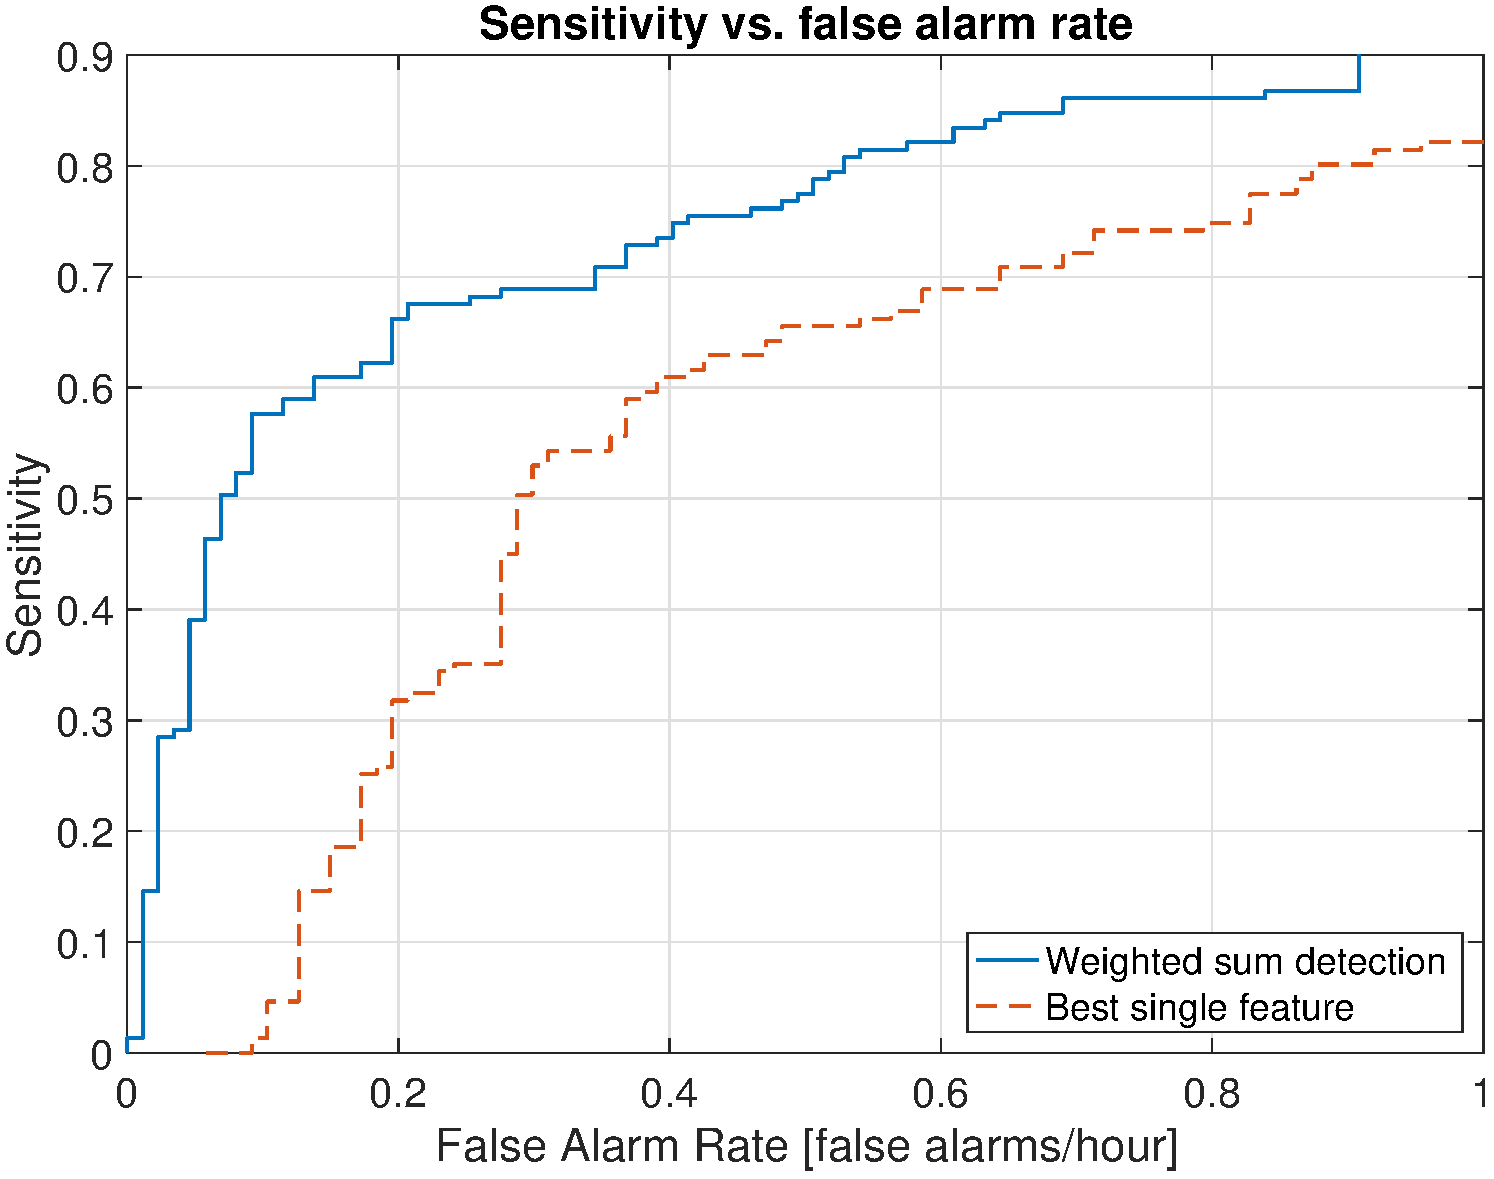
\includegraphics[width = 0.6\textwidth]{img/characteristic_curve}
	\caption{An exemplary operating characteristic plot.}
	\label{fig:roc}
\end{figure}

The properties of the \verb|OperatingCharacteristicCurve| class  properties are:

\begin{center}
	\begin{longtable}{p{5cm}|p{12cm}}
	\textbf{Name:} & \textbf{Description:} \\ \hline
	\verb|Name| & name of the object, used to identify the curve once plotted in the plot legend \\
	\verb|Sensitivity| & a vector that holds the sensitivity values for different thresholds \\
	\verb|FalseAlarmRate| & a vector of that holds the false alarm rates for different thresholds \\
	\verb|ThresholdFactor| & a vector that holds the thresholds (or threshold factor values) corresponding the sensitivities and false alarm rates in the above properties \\
	\verb|Area| & area under the curve 
	\end{longtable}
\end{center}

The constructor for this class is 
\begin{Verbatim}
	curve = OperatingCharacteristicCurve(name, sensitivity, falseAlarmRate, threshold)
\end{Verbatim}
where the first input argument is a char and the last three input arguments are vectors of the same size. \\

The characteristic curve can be plotted by calling \verb|plot()|. This will create a new figure with the characteristic curve plotted in it. The function \verb|plot()| returns two output arguments. The first is a handle to the newly created figure and the second one is a handle to the axis that contains the curve.

The function \verb|addCurve(h)| can be called to add the curve contained in this object to an already existing plot. The input argument \verb|h| is a handle to figure or to the axes containing the already existing curves. 

Both the \verb|plot| and \verb|addCurve| function can take an additional extra input argument that specifies the name under which the curve will appear in the legend. If this is not specified, the name in the legend will be the \verb|Name| property of the object. For example, the plot in figure \ref{fig:roc} was created by
\begin{Verbatim}
	[h, ax] = dummyObject1.plot('Weighted sum detection');
	dummyObject2.addCurve(h, 'Best single feature');	
\end{Verbatim}

Finally, the function \verb|calculateArea(upperBound)| calculates the area under the curve between a false alarm rate of 0 and the false alarm rate specified by input argument \verb|upperBound| and returns it. The input argument can be omitted, in which case it is defaulted to 1.


%--------------------------------------------------------------------
\newpage
\section{Other functions}

Some (but not all) of the other available functions are described in this section.

\subsection{iEEG\_getData function} \label{sec:ieeg_getdata}

The \verb|IEEG_getData| function is used to download data from the iEEG.org website. 
\begin{Verbatim}
	measurement = IEEG_getData(studyName, channel, loginName, loginBin)
\end{Verbatim}
It has 4 required input arguments and return an instance of the \verb|Measurement| class that contains all relevant information about the recording (seizure start and end, sampling frequency, ...). The required input arguments are in order:
\begin{enumerate}
	\item \verb|studyName| is a char that must correspond to the name of the iEEG.org study that is to be downloaded
	\item \verb|channel| is a double that corresponds to the number of the channel that is to be downloaded
	\item \verb|loginName| is a char that corresponds to the User ID that is used to login to the iEEG.org website
	\item \verb|loginBin| is a path to the \verb|.bin| file that holds the password that is used to login to the iEEG.org website. Please see the iEEG.org MATLAB Toolbox documentation for more details about what this is.
\end{enumerate}

\subsection{MatrixCrossValidation function}

The \verb|MatrixCrossValidation| function performs $k$-Fold cross-validation on a \verb|MatrixDetection| class.

\begin{Verbatim}
	[curves_training, curves_validation] = MatrixCrossValidation(...
    	matrix, chunkSize_minutes, numFolds)
\end{Verbatim}
It has 4 required input parameters:
\begin{itemize}
	\item \verb|matrix|: a \verb|FeatureMatrix| object
	\item \verb|chunkSize_minutes|: the length in minutes of one chunk
	\item \verb|numFolds|: the number of folds the data is divided into
\end{itemize}
It returns two cell arrays \verb|curves_training| and \verb|curves_training| of length \verb|numFolds|. 

The data is first divided into chunks of \verb|chunkSize_minutes| length. Seizures are not being divided, so some chunks might be slightly longer than that duration, since if a seizure is at the edge of one chunk, the chunk is extended so that the whole seizure is inside the chunk. The chunks are then shuffled. 

The matrix seizure detection algorithm is then trained on \verb|1-1/numFolds| parts of the data and tested on the \verb|1/numFolds| remaining part. This is repeated \verb|numFolds| times, changing the part of the data that is used for training and testing for every iteration. The data from the original \verb|FeatureMatrix| passed as input argument is split into the training and testing part using the \verb|cut| function of the \verb|FeatureMatrix| class (this function is not documented in the user guide).

Two \verb|MatrixDetection| objects are created, one for training and one for testing. The training consists of calculating all the optimal thresholds for all features inside the feature matrix, their weights and the optimal threshold for the \verb|MatrixDetection| object. This is done only on the training data. All these thresholds and weights are then transferred to the second \verb|MatrixDetection| object and the detection is then evaluated using the testing data. The operating characteristic curves of both the training and the testing \verb|MatrixDetection| objects are saved and returned at the end of the function. \\

Currently, the detection algorithm being cross-validated is the one implemented in \texttt{MatrixDetection\_Linear\-Regression}. Thus, the training object is actually a \verb|MatrixDetection_LinearRegression| object. To change the algorithm being cross-validated, the relevant section has to be changed inside the function. The testing object is always a \verb|MatrixDetection| object because no weights are computed for the testing object, they are just copied over from the training object.


%--------------------------------------------------------------------
\newpage
\appendix
\section{Appendix} 

\subsection{Feature Calculation Formulas} \label{sec:formulas}

The different feature are calculated based on the formulas described below. The sliding window has a length of $N$ samples and $x[n]$ represents the $n$th sample of every window.
\begin{itemize}
	\item \textbf{Line Length} $$ \sum_{i=2}^N \Big|x[i] - x[i-1]\Big|$$
	\item \textbf{Nonlinear Energy} $$\frac{1}{N-2} \sum_{i=2}^{N-1} x[i]^2 - x[i-1]x[i+1]$$
	\item \textbf{Full Spectrum Power} $$\frac{1}{N} \sum_{i=1}^N x[i]^2$$
	\item \textbf{Spectral band power in the theta band}: same as full spectrum power but the data is first filtered using a Butterworth bandpass filter with cutoff frequencies 4 Hz and 8 Hz
	\item \textbf{Spectral band power in the alpha band}: same as full spectrum power, the data was first filtered using a Butterworth bandpass filter with cutoff  frequencies 8 Hz and 14 Hz
	\item \textbf{Spectral band power in the beta band}: same as full spectrum power, the data was first filtered using a Butterworth bandpass filter with cutoff  frequencies 14 Hz and 32 Hz \\
\end{itemize}

\subsection{Metrics definition} \label{sec:metrics}

The sensitivity is defined as 
$$\text{sensitivity} = \frac{\text{number of seizures detected}}{\text{total number of seizures}}.$$

The specificity is defined as
$$\text{specificity} = \frac{\text{number of interictal feature samples below threshold}}{\text{total number of interictal feature samples}}$$ where an interictal feature sample is a feature sample that does not correspond to a seizure.

%%%%%%%%%%%%%%%%%%%%%% END DOCUMENT %%%%%%%%%%%%%%%%%%%%%%%%%%%%%%
\end{document}
